\documentclass{article}

\def\showtopic{Numerical Analysis}
\def\showtitle{Lab 1: Interpolation}
\def\showabs{Lab 1}
\def\showauthor{Ting Lin, 1700010644}
\usepackage{amsmath, amsfonts, amsthm}

\usepackage{graphicx, epstopdf}
\usepackage{color}
\usepackage{geometry, graphicx}
\usepackage{algorithm, algorithmic}
\usepackage{bm}
\usepackage{multirow}
\usepackage{ulem}
\geometry{left = 5em, right = 5em}
\usepackage{listings}
\usepackage{xcolor}
%% notation macro
\newcommand{\F}{\mathcal F}
\newcommand{\T}{\mathcal T}
\newcommand{\I}{\mathcal I}
\newcommand{\U}{\mathcal U}
\newcommand{\R}{\mathbb R}
\renewcommand{\P}{\mathcal P}
\newcommand{\uP}{ \mathcal \uline P}
\newcommand{\B}{\mathcal B}
%\newcommand{\R}{\mathbb R^2}
\newcommand{\Z}{\mathbb Z}
\newcommand{\C}{\mathbb C}
\newcommand{\laplacian}{\triangle}
\newcommand{\grad}{\nabla}
\renewcommand{\div}{\textrm{div~}}

\newcommand{\diff}[2]{\frac{\partial #1}{\partial #2}}
\newcommand{\difff}[3]{\frac{\parial #1^2}{\partial #2 \partial #3}}
\newcommand{\diFF}[2]{\frac{\partial #1^2}{\partial^2 #2}}
\newcommand{\diam}{\text{ diam }}
%% non-noation macro
\newcommand{\IN}{\text{  in  }}
\newcommand{\ON}{\text{  on  }}
\newcommand{\st}{\text{s.t.  }}
\newcommand{\tbc}{{\color{red}[TBC]}}

%% enviorment
\newtheorem{proposition}{Proposition}
\newtheorem{definition}{Definition}
\newtheorem{corollary}{Corollary}
\newtheorem{remark}{Remark}



\title{\textbf{\showtitle}}
\author{\showauthor}
\usepackage{indentfirst}
\usepackage{fancyhdr}  
\pagestyle{fancy}
\lhead{\textbf {\showtopic} }
\chead{} 
\rhead{\textbf {\showabs} }
\lfoot{} 
\cfoot{\thepage}
\rfoot{} 
\renewcommand{\headrulewidth}{0.4pt} 
\renewcommand{\u}{\uline u}
\renewcommand{\v}{\uline v}
\newcommand{\n}{\uline n}
\newcommand{\f}{\uline f}
\newcommand{\eps}{\uuline \varepsilon}
\begin{document}
	\maketitle
	\thispagestyle{fancy}
	\tableofcontents
	
	\section*{}
In this report we will focus on various type of interpolation formulas: Lagrange, Newton, piecewise linear, Hermite and (cubic) spline. We will show the algorithms and theoretical analysis (mainly error estimation). In numerical experiments, we will show several numerical result and discuss what causes Runge's phenomenon briefly.

We first introduce the problem setting, suppose $f(x)$ is a continuous function on an interval $I$, and $x_0,\cdots, x_n$ be $n$ distinct points, (called interpolation nodes or nodes throughout this paper) we aim to find a simple function $p$ such that $p(x_i) = f(x_i)$. There are some principles to determine a proper $p$: First, $p$ should be easily derived from the information of $f$ and nodes. Second, for a given point $x$, the value $p(x)$ can be computed easily. Third and most essentially, the error between $f(x)$ and $p(x)$ are rather small (under some measure).

\section{Lagrange and Newton Interpolation}
\subsection{Lagrange Interpolation Formula}
We first consider a global polynomial to interpolate. The task is to find a polynomial of degree $n$ such that 
$$p(x_i) = f(x_i)$$ for each $x_i$. The existence and uniqueness can be reduced to a linear system, which coefficient matrix is 
Vandermonde-like. Since a Vandermonde matrix is invertible, we conclude there exists a unique polynomial satisfying our needs. 

There is also a explicit formula, called Lagrange interpolation formula.

$$p(x) = \sum_{i=0}^n f(x_i)l_i(x) = \sum_{i=0}^n f(x_i) \prod_{j\neq i} \frac{x - x_j}{x_i - x_j}.$$

Here $l_i(x_j) = \delta_{ij}$ can be thought as a dual basis. Clearly the construction is correct at each interpolation node. 

Now we show the remainder estimates of Largrange Polynomial.

\begin{proposition}
	Suppose $f(x) \in C^{n+1}[a,b]$, then $\forall x \in [a,b]$, $\exists \xi \in [a,b]$, such that the remainder term $$R(x) = f(x) - p(x) = \frac{f^{n+1}(\xi)}{(n+1)!}\prod_{i = 0}^n(x-x_i).$$
\end{proposition}
\subsection{Newton's Formula}
We shall give another expression of Lagrange Interpolation, which is called Newton interpolation. To describe the idea precisely, we first introduce the concept of difference quotients.

$$f[x_j] = f(x_j) \qquad j = 0,1,\cdots,n$$
$$f[x_j,\cdots, x_{j+k}] = \frac{f[x_{j+1},\cdots, f_{j+k}] - f[x_{j},\cdots, f_{j+k-1}]}{x_{j+k} - x_j}$$
Then we have 
$$p(x) = f[x_0] + f[x_0,x_1](x-x_0) + \cdots f[x_0, \cdots, x_n](x-x_0)\cdots (x-x_{n_1}),$$
which coincidences with Lagrange interpolation. 


For evaluation procedure, we use Horner's rule to reduce the computational step.
Based on Newton interpolation, we have another error estimates, which reduce the requirement of regularity. 
\begin{proposition}
	With $f$ no regularity, we have 
	$$R(x) = f[x,x_0, \cdots, x_n] (x-x_0) \cdots (x-x_n).$$ 
\end{proposition}
Notice that from this representation formula, we can also derive the error estimates in the previous subsection. 
\section{Piecewise Polynomial Interpolation}
In many case, the global polynomial is not satisfactory. Hence we turn to find a interpolation formula using piecewise polynomial. The advantage of piecewise polynomial is that we can capture and express the behavior of function more accurate. For simplicity, when $x \in [x_0, x_{n}]$ the interpolation becomes vacuous. 
\subsection{Piecewise Linear Interpolation}
The most simple case is piecewise linear interpolation. Let $p(x)$ be a function that 
$$p(x) = \frac{x-x_i}{x_{i+1}-x_i}f(x_{i+1}) + \frac{x-x_{i+1}}{x_{i}-x_{i+1}}f(x_i)$$
whenever $x \in [x_i, x_{i+1}]$.

We can easily derive the error estimates. 
\begin{proposition}
	Suppose $f \in C^2[a,b]$, then 
	$$|f(x) - p(x)| \le \frac{Mh^2}{8},$$
	where $M = |f|_{C^2[a,b]}$, $h = \max {x_{i+1} - x{i}}$.
\end{proposition}

\subsection{Hermite Interpolation}
Consider a little more complicated case when we use piecewise cubic polynomial to interpolate. Suppose we know the value of $f'(x_i)$ additionally, then in each interval $[x_i, x_{i+1}]$, the following condition determines a polynomial.

$$p(x_k) = f(x_k),\quad p'(x_k) = f'(x_k), k = i,i+1$$
on each interval $[x_i, x_{i+1}]$.

Simple calculation yields a basis of this type of interpolation. 

\begin{equation}
\begin{split}
p(x) &= f(x_i)(1+2\frac{x-x_i}{x_{i+1} - x_i})(\frac{x-x_{i+1}}{x_i - x_{i+1}})^2 + f(x_{i+1})(1+2\frac{x-x_{i+1}}{x_i - x_{i+1}})(\frac{x-x_i}{x_{i+1} - x_i})^2\\
&+f'(x_{i})(x-x_i)(\frac{x-x_{i+1}}{x_i - x_{i+1}})^2 + f'(x_{i+1})(x-x_{i+1})(\frac{x-x_i}{x_{i+1} - x_i})^2
\end{split}
\end{equation}
on each interval. 

The error estimates are analogous to that we obtained in the previous subsection.

\begin{proposition}
	Suppose $f \in C^4[a,b]$, then 
	$$|f(x) - p(x)| \le \frac{Mh^4}{384},$$
	where $M = |f|_{C^4[a,b]}$, $h = \max {x_{i+1} - x{i}}$.
\end{proposition}

\subsection{Cubic Spline Interpolation}
The cubic spline interpolation is similar to Hermite interpolation but the derivatives of interpolation nodes is replaced by a second-order continuity. More precisely we aim to find a global $C^2$ function, whose restriction on $[x_i, x_{i+1}]$ is cubic. Under natural BC (i.e. $p''(x_0) = p''(x_n) = 0$), the derivatives of each node can be derived through the following linear system, using the inter node $C^2$ continuity :

\begin{equation}
\begin{bmatrix}
2 &\lambda_0& 0 & \cdots & 0\\
1 - \lambda_1 & 2 & \lambda_1  & & \vdots\\
0 & \ddots &\ddots & \ddots & 0 \\
\vdots &  &  1-\lambda_{n-1}  & 2 & \lambda_{n_1} \\ 
0 & \cdots & 0 & 1-\lambda_n & 2
\end{bmatrix}
\begin{bmatrix}
p'(x_0)\\
p'(x_1)\\
\vdots\\
p'(x_{n-1})\\
p'(x_n)
\end{bmatrix} = 
\begin{bmatrix}
\mu_0\\
\mu_1\\
\vdots\\
\mu_{n-1}\\
\mu_n
\end{bmatrix}
\end{equation}

Where 
$$\Delta x_{i} = x_{i+1} - x_{i}$$
$$\lambda_i = \frac{\Delta x_i}{\Delta x_{i-1} + \Delta x_i}, \quad i = 1,2,\cdots, n-1$$
$$\mu = 3 [ \frac{1 - \lambda_i}{\Delta x_{i_1}}(f(x_i) - f(x_{i_1})) + \frac{ \lambda_i}{\Delta x_{i}}(f(x_{i+1}) - f(x_i))] \quad i = 1,2,\cdots, n-1$$

For corner case, we set $\lambda_0 = 1, \lambda_n = 0$, $ \mu_0 = 3[\frac{f(x_1) - f(x_0)}{\Delta x_0}], \mu_n = 3[\frac{f(x_n) - f(x_{n-1})}{\Delta x_{n-1}}]$. 

Then $p'(x_i)$ can be solved by Thomas' method, after that we use classical Hermite Interpolation with $p'(x_i)$ being derivatives.

\section{Implementation}
In this section we briefly discuss the implementation details, see the source code for further. 
\paragraph{Lagrange}: All we need is to compute the basis function.
\paragraph{Newton}: We first compute the different quotient sequentially, then apply Horner's rule to reduce computational complexity.
\paragraph{Piecewise Linear and Hermite}:  Faced numerous inputs, we use two list to store nodes $N$ and inputs $X$. We scan $X$ and use an index to record its located interval. 
\section{Numerical Results}
In this report we show the numerical experiments. 
\subsection{Questions}
\begin{figure}[h]
	\centering
	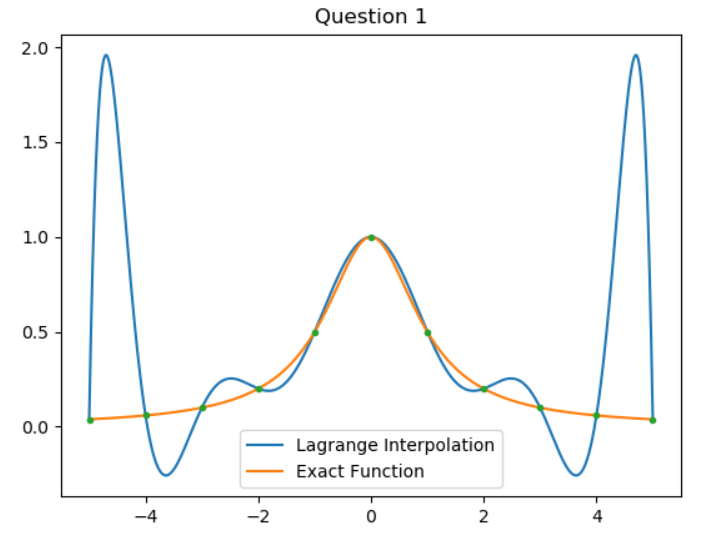
\includegraphics[scale=.5]{../fig/q1.png}
\end{figure}
\begin{figure}[h]
	\centering
	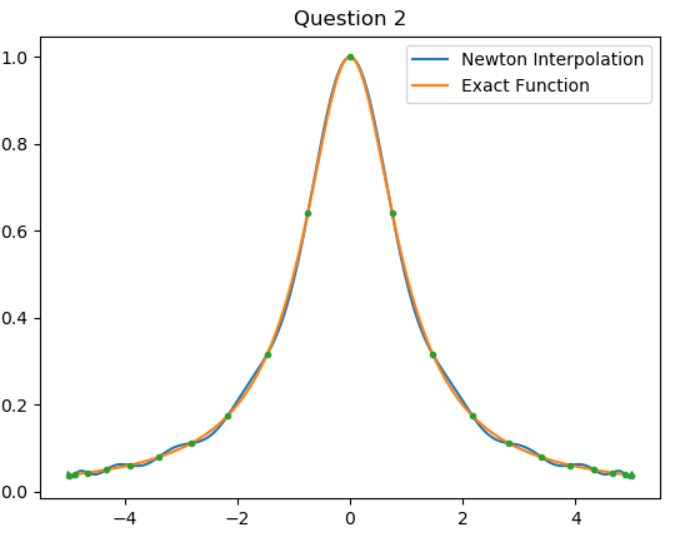
\includegraphics[scale=.5]{../fig/q2.png}
\end{figure}
\begin{figure}[h]
	\centering
	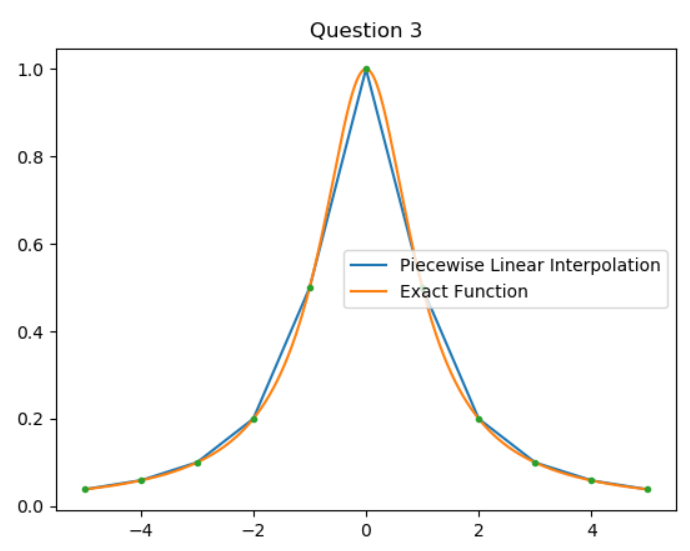
\includegraphics[scale=.5]{../fig/q3.png}
\end{figure}
\begin{figure}[h]
	\centering
	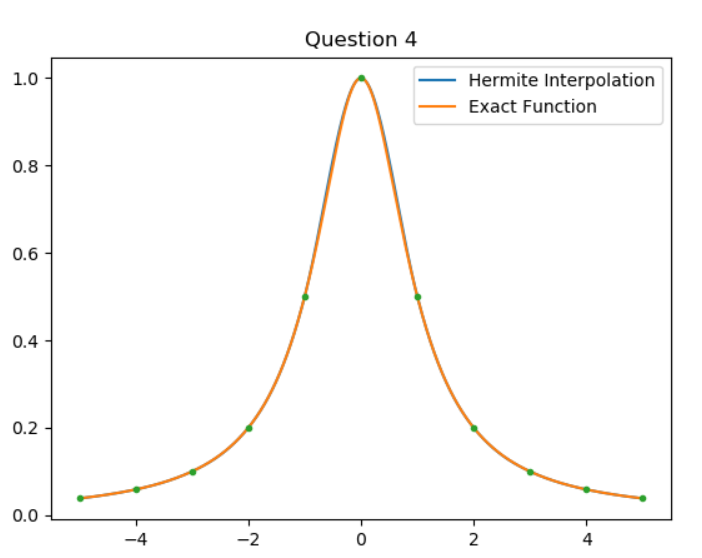
\includegraphics[scale=.45]{../fig/q4.png}
\end{figure}
\begin{figure}[h]
	\centering
	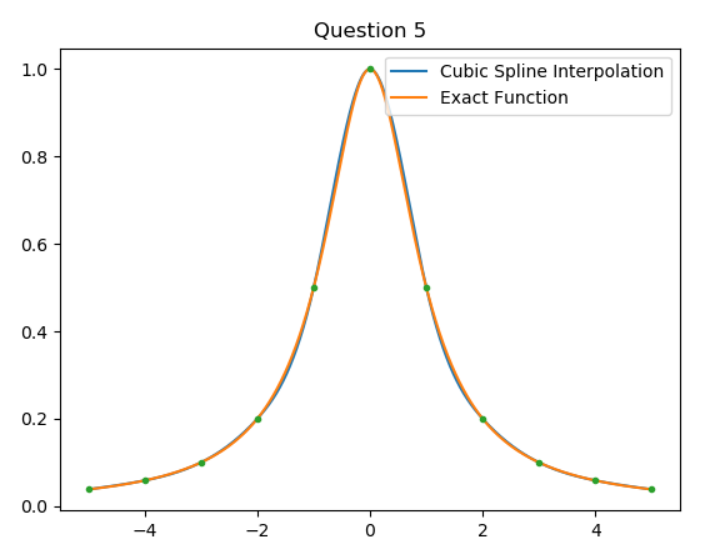
\includegraphics[scale=.45]{../fig/q5.png}
\end{figure}


We show several figures demonstrate the interpolation methods and results, corresponding to each question. Additionally, we compare the error between the Hermite method and cubic spline method. 
\begin{figure}[h]
	\centering
	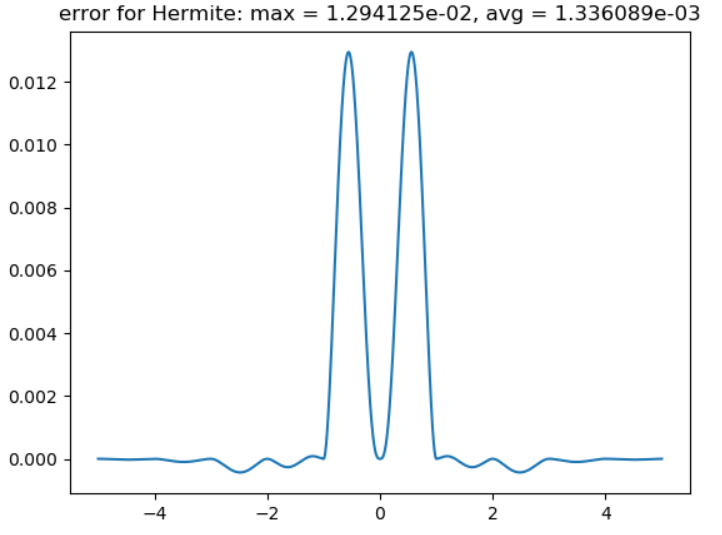
\includegraphics[scale=.3]{../fig/err.png}
	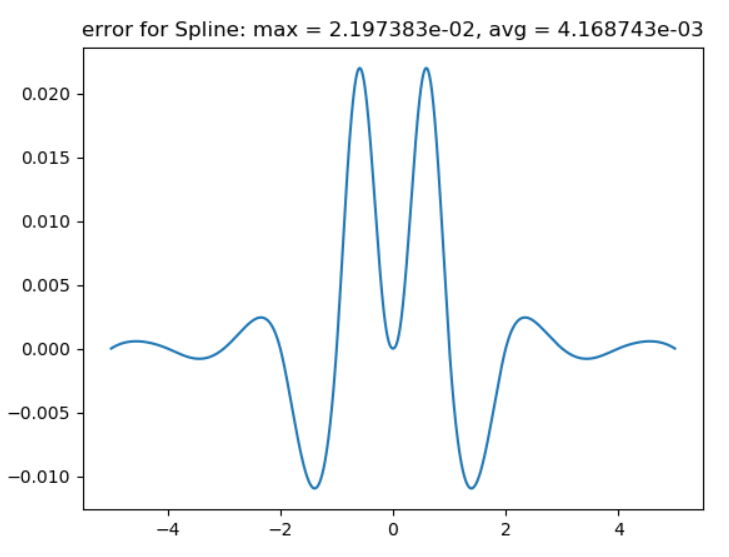
\includegraphics[scale=.3]{../fig/err5.png}
	\caption{The interpolation error of Hermite and Cubic spline methods.}
\end{figure}

\subsection{Discussions}

From the figure we can know that in this situation things are better when Hermite method is used. However, more condition like derivatives is required, which is laborious or even impossible to obtain in real application. So cubic spline meets the practical demand. 

Now we turn to the first two examples which uses the same global polynomial interpolation but with different node sets. They differs much as we see.  This is called Runge's phenomena. Ideally, this can be remedied by a good interpolation nodes set.


\end{document}
















Escape special TeX symbols (%, &, _, #, $)